% =============================================================================
\chapter{Quantum noise in BEC interferometry}
\label{cha:bec-noise}
% =============================================================================

BECs are macroscopic quantum objects and can be potentially used as high precision interferometric detectors and sensors.
Unlike photons, atoms can interact strongly, leading to loss of coherence and decreased interferometric contrast.
An accurate quantitative model for these quantum many-body effects is essential for explaining the results of atom interferometry experiments and for planning the future ones.

In this chapter we will apply the truncated Wigner method from \charef{wigner-bec} to the task of simulating the dynamics of such experiments.
We will start from describing the mean-field approach leading to the conventional Gross-Pitaevskii equations~\cite{Pitaevskii2003} (\abbrev{gpe}s).
We then extend it to include quantum effects, such as the noise from linear and nonlinear losses.
The accurate description of nonlinear losses is especially important as their relative effect increases when atom numbers are increased to improve contrast.

We will compare the effect of quantum fluctuations and technical noises, such as imperfect measurements or coupling phase and amplitude uncertainty, on the interferometric contrast.
We will also consider the experimental measurement process of the contrast in detail and investigate the influence of quantum effects on such an important characteristic as phase noise.

% =============================================================================
\section{Two-component trapped BEC}
\label{sec:bec-noise:system}
% =============================================================================

The system we are interested in is an ultracold harmonically trapped \Rb{} \abbrev{bec} in $3$ effective dimensions such as the one used in the experiments by Riedel \textit{et~al}~\cite{Riedel2010} and Egorov \textit{et~al}~\cite{Egorov2011,Egorov2013}.
The \abbrev{bec} in question has two components, with a significant nonlinear repulsive interaction (both inter- and intra-component), nonlinear losses and perhaps some additional linear unitary effects, such as electromagnetic coupling between components.
The number of components is only set to two in order to simplify resulting equations for the experiments described in this chapter; it can be easily increased if necessary.

We assume that the \abbrev{bec} has $s$-wave interactions, which makes the nonlinear interaction coefficients have the form
\begin{eqn}
\label{eqn:bec-noise:system:g}
    g_{jk} = \frac{4\pi\hbar^2 a_{jk}}{m},
\end{eqn}
where $j$ and $k$ are the indexes of the interacting components, $a_{jk}$ is the corresponding $s$-wave scattering length, and $m$ hereinafter in this chapter stands for the atom mass of \Rb{}.
Here we assume a momentum cutoff $k_d \ll 1 / a_{jk}$ in the numerical simulations, otherwise the couplings must be renormalized~\cite{Sinatra2002}.

The external harmonic trapping potential $V_j$ for the component $j$ (which can include a component-dependent shift along some of the axes) has the form
\begin{eqn}
\label{eqn:bec-noise:system:V}
    V_j
    = \frac{m}{2} \sum_{d=1}^3 \omega_d^2 (x_d - l_d)^2,
\end{eqn}
where $\omega_d$ are trapping frequencies, which will be specified later when the concrete experiments are described.

Again, in principle, the methods described in this chapter can be easily generalized to include an arbitrary potential shape, and possibly some different form of nonlinear interaction coefficients, but for the experiments to be described the equations above will apply.

% =============================================================================
\section{Mean-field approximation}
\label{sec:bec-noise:mean-field}
% =============================================================================

We will start from a classical model of a trapped \abbrev{bec}~--- the mean-field approximation.
While it cannot predict quantum effects, it provides the basis for comparison with the truncated Wigner method, and can be also applied to calculate the ground state of a trapped \abbrev{bec} numerically.

We will use the combined model which includes linear coupling and losses, and later in \secref{bec-noise:wigner}, dedicated to the application of the truncated Wigner method we will show how we can get almost identical equations from the first principles.


% =============================================================================
\subsection{Two-component condensate}
% =============================================================================

In the mean-field approximation the two-component \abbrev{bec} is described by wavefunctions $\Psi_j$, which are normalized such that $\int |\Psi_j|^2 \upd\xvec \equiv N_j$, where $N_j$ is the total population of the component $j$ (consequently, $|\Psi_j|^2 \equiv n_j$ is the component density).
The evolution of the condensate is described by the system of coupled Gross-Pitaevskii equations (\abbrev{cgpe}s)~\cite{Pitaevskii2003}
\begin{eqn}
\label{eqn:bec-noise:mean-field:cgpes}
	i \hbar \frac{\upd \Psi_1}{\upd t} ={} & \left(
		-\frac{\hbar^2 \nabla^2}{2 m} + V_1
		+ g_{11} \lvert \Psi_1 \rvert^2
		+ g_{12} \lvert \Psi_2 \rvert^2
		- i \hbar \Gamma_1
	\right) \Psi_1 \\
	& + \frac{\hbar \Omega}{2} \left(
		e^{i (\omega t + \alpha)} + e^{-i (\omega t + \alpha)}
	\right) \Psi_2, \\
	i \hbar \frac{\upd \Psi_2}{\upd t} ={} & \left(
		-\frac{\hbar^2 \nabla^2}{2 m} + V_2 + \hbar \omega_{hf}
		+ g_{22} \lvert \Psi_2 \rvert^2
		+ g_{12} \lvert \Psi_1 \rvert^2
		- i \hbar \Gamma_2
	\right) \Psi_2 \\
	& + \frac{\hbar \Omega}{2} \left(
		e^{i (\omega t + \alpha)} + e^{-i (\omega t + \alpha)}
	\right) \Psi_1.
\end{eqn}
Here $V_j(\xvec)$ are external potentials~\eqnref{bec-noise:system:V}, $\omega_{hf}$ is the hyperfine splitting between components, $g_{jk}$ are nonlinear interaction coefficients~\eqnref{bec-noise:system:g}, $\Gamma_j$ terms represent nonlinear losses for the component $j$, and $\Omega$ is the electromagnetic coupling strength (with $\omega$ being the frequency, and $\alpha$ the initial phase shift of the coupling).
The \abbrev{cgpe}s without loss or coupling terms were introduced by Zeng \textit{et~al}~\cite{Zeng1995}, and Ho and Shenoy~\cite{Ho1996}.
The coupling terms were first included by Ballagh \textit{et~al}~\cite{Ballagh1997}, and the loss terms by Yurovsky \textit{et~al}~\cite{Yurovsky1999}.
A detailed description of the mean-field approximation can be found in the book by Pitaevskii and Stringari~\cite{Pitaevskii2003}.

The exact expressions for the loss parameters $\Gamma_j$ depend on the loss processes in a particular experiment.
For example, the dominant three-body and two-body losses in a two-component \Rb{} \abbrev{bec} with the components ${\ket{F=1,\, m_F=-1}}$ and ${\ket{F=2,\, m_F=+1}}$ result in~\cite{Burt1997,Mertes2007}
\begin{eqn}
\label{eqn:bec-noise:mean-field:losses}
	\Gamma_1 &= \left( \gamma_{111} n_1^2 + \gamma_{12} n_2 \right) / 2, \\
	\Gamma_2 &= \left( \gamma_{12} n_1 + \gamma_{22} n_2 \right) / 2.
\end{eqn}
These equations were obtained empirically, but we will see later in this chapter how the same expressions (to leading order) appear as a result of the application of the truncated Wigner method.

The coupling frequency $\omega$ is usually slightly detuned from the hyperfine frequency in the experiment: $\omega = \omega_{hf} + \delta$, where $\delta \ll \omega_{hf}$.
It is convenient to use equations~\eqnref{bec-noise:mean-field:cgpes} in a rotating frame:
\begin{eqn}
	\Psi_1 & = \Psi_1^{(r)}, \\
	\Psi_2 & = \Psi_2^{(r)} e^{i \omega_{hf} t}.
\end{eqn}
This transformation eliminates $\omega_{hf}$ from the equations and does not change single-time observable values.
Dropping the rotating frame superscript for simplicity, we obtain the transformed equations
\begin{eqn}
	i \hbar \frac{\upd \Psi_1}{\upd t} ={} & \left(
		-\frac{\hbar^2 \nabla^2}{2 m} + V_1
		+ g_{11} \lvert \Psi_1 \rvert^2
		+ g_{12} \lvert \Psi_2 \rvert^2
		- i \hbar \Gamma_1
	\right) \Psi_1 \\
	& + \frac{\hbar \Omega}{2} \left(
		e^{i ((\omega + \omega_{hf}) t + \alpha)} + e^{-i (\delta t + \alpha)}
	\right) \Psi_2, \\
	i \hbar \frac{\upd \Psi_2}{\upd t} ={} & \left(
		-\frac{\hbar^2 \nabla^2}{2 m} + V_2
		+ g_{22} \lvert \Psi_2 \rvert^2
		+ g_{12} \lvert \Psi_1 \rvert^2
		- i \hbar \Gamma_2
	\right) \Psi_2 \\
	& + \frac{\hbar \Omega}{2} \left(
		e^{i (\delta t + \alpha)} + e^{-i ((\omega + \omega_{hf}) t + \alpha)}
	\right) \Psi_1.
\end{eqn}

Furthermore, in experiments the coupling field is typically applied for short periods of time $t_{\mathrm{pulse}}$, where $1 / \omega \ll t_{\mathrm{pulse}} \ll 1 / \delta$.
This allows us to neglect the rapidly oscillating terms proportional to $e^{i(\omega + \omega_{hf})t}$ and come to \abbrev{cgpe}s in the rotating frame:
\begin{eqn}
\label{eqn:bec-noise:mean-field:cgpes-simplified}
	i \hbar \frac{\upd \Psi_1}{\upd t} & = \left(
		-\frac{\hbar^2 \nabla^2}{2 m} + V_1
		+ g_{11} \lvert \Psi_1 \rvert^2
		+ g_{12} \lvert \Psi_2 \rvert^2
		- i \hbar \Gamma_1
	\right) \Psi_1
	+ \frac{\hbar \Omega}{2} e^{-i (\delta t + \alpha)} \Psi_2, \\
	i \hbar \frac{\upd \Psi_2}{\upd t} & = \left(
		-\frac{\hbar^2 \nabla^2}{2 m} + V_2
		+ g_{22} \lvert \Psi_2 \rvert^2
		+ g_{12} \lvert \Psi_1 \rvert^2
		- i \hbar \Gamma_2
	\right) \Psi_2 +
	\frac{\hbar \Omega}{2} e^{i (\delta t + \alpha)} \Psi_1.
\end{eqn}
When the pulse is applied twice using the same coupling field (which is the case for the Ramsey interferometry), it is the same as just setting $\Omega$ to zero after the first pulse and then restoring its value for the time of the second pulse; therefore, $\alpha$ stays the same too.
If one wants to apply pulse with the different detuning, the phase information is lost, and the value of $\alpha$ has to be regarded as random.

The application of the coupling field can be simplified when certain additional conditions are valid, namely:
\begin{itemize}
	\item $\mu / \hbar \ll \Omega$, where $\mu$ is the chemical potential of the first component;
	\item $\delta \ll \Omega$;
	\item the characteristic time of the other terms in~\eqnref{bec-noise:mean-field:cgpes} is much greater than $t_{\mathrm{pulse}}$.
\end{itemize}
This allows us to use an ``instantaneous'' pulse, multiplying the state vector by a rotation matrix:
\begin{eqn}
\label{eqn:bec-noise:mean-field:rotation-matrix}
	\begin{pmatrix}
		\Psi^\prime_1 \\ \Psi^\prime_2
	\end{pmatrix} =
	\begin{pmatrix}
		\cos \frac{\theta}{2} & -i e^{-i \phi} \sin \frac{\theta}{2} \\
		-i e^{i \phi} \sin \frac{\theta}{2} & \cos \frac{\theta}{2}
	\end{pmatrix}
	\begin{pmatrix}
		\Psi_1 \\ \Psi_2
	\end{pmatrix},
\end{eqn}
where $\theta = \Omega t_{\mathrm{pulse}}$, and $\phi = \delta t + \alpha$ is the total phase of the coupling field at the beginning of the pulse.
In particular, for the two-pulse Ramsey scheme (\figref{bec-noise:visibility:sequences},~(a)) with the time $t_R$ between pulses, $\phi_2 = \phi_1 + \delta t_R$.


% =============================================================================
\subsection{Ground state calculation}
% =============================================================================

At the beginning of the simulation, the \abbrev{bec} is assumed to be in the ground state which has the lowest possible energy.
The ground state is the solution of the stationary \abbrev{cgpe}s
\begin{eqn}
\label{eqn:bec-noise:mean-field:cgpes-stationary}
	\mu_1 \Psi_1 & = \left(
		-\frac{\hbar^2 \nabla^2}{2 m} + V_1
		+ g_{11} \lvert \Psi_1 \rvert^2
		+ g_{12} \lvert \Psi_2 \rvert^2
	\right) \Psi_1, \\
	\mu_2 \Psi_2 & = \left(
		-\frac{\hbar^2 \nabla^2}{2 m} + V_2
		+ g_{22} \lvert \Psi_2 \rvert^2
		+ g_{12} \lvert \Psi_1 \rvert^2
	\right) \Psi_2,
\end{eqn}
where $\mu_1$ and $\mu_2$ are chemical potentials of the components.

The most common method of finding the mean-field ground state is the imaginary time propagation~\cite{Chiofalo2000,Bao2004}.
The essence of the method is that the propagation of an arbitrary wavefunction using the time-dependent \abbrev{cgpe}s, but with the substitution $t \rightarrow \tau = it$, lowers its energy; therefore, after the sufficient amount of time this propagation will lead us arbitrarily close to the ground state.
The actual equations to be propagated are~\eqnref{bec-noise:mean-field:cgpes-simplified} without the loss or coupling terms:
\begin{eqn}
\label{eqn:bec-noise:mean-field:imaginary-time}
	\hbar \frac{\upd \Psi_1}{\upd \tau} & = -\left(
		-\frac{\hbar^2 \nabla^2}{2 m} + V_1
		+ g_{11} \lvert \Psi_1 \rvert^2
		+ g_{12} \lvert \Psi_2 \rvert^2
	\right) \Psi_1, \\
	\hbar \frac{\upd \Psi_2}{\upd \tau} & = -\left(
		-\frac{\hbar^2 \nabla^2}{2 m} + V_2
		+ g_{22} \lvert \Psi_2 \rvert^2
		+ g_{12} \lvert \Psi_1 \rvert^2
	\right) \Psi_2.
\end{eqn}

The rigorous proof of this method was derived by Bao and Du~\cite{Bao2004}.
The idea can be roughly illustrated by considering a one-component system with a linear Hamiltonian $\hat{H}$, whose eigenvalues are $\mu_1 < \mu_2 < ...$, where the lowest eigenvalue corresponds to ground state we want to find.
The steady solution of the time-dependent \abbrev{gpe}
\begin{eqn}
	i \hbar \frac{\upd \Psi}{\upd t} = \hat{H} \Psi
\end{eqn}
then looks like
\begin{eqn}
	\Psi(\xvec, t) = \sum_k e^{-\frac{i}{\hbar}\mu_k t} f_k(\xvec),
\end{eqn}
where $f_k$ are eigenfunctions of $\hat{H}$ corresponding to the eigenvalues $\mu_k$.
After the substitution $t \rightarrow \tau = it$ the solution becomes fading, with higher-energy terms fading faster:
\begin{eqn}
	\Psi(\xvec, \tau) = \sum_k e^{-\frac{1}{\hbar}\mu_k \tau} f_k(\xvec).
\end{eqn}

Therefore, if we take some random initial solution and propagate it long enough in imaginary time using~\eqnref{bec-noise:mean-field:imaginary-time}, the higher-energy terms will eventually die out (in comparison with the lowest-energy state) and leave us with the desired ground state.
The state obtained from the Thomas-Fermi approximated \abbrev{gpe} can be taken as the initial one since it is rather close to the desired one (and, therefore, higher-energy terms are already quite small).

Since the population will decrease exponentially after each step, and the precision of numerical calculations is limited, a renormalisation after each step will be required.
The total number of atoms in the ground state serves best in this case (because we will have to renormalise the final ground state anyway):
\begin{eqn}
	\int\limits_V \lvert \Psi(\tau, \xvec) \rvert^2 \upd V = N.
\end{eqn}

Propagation is terminated when the Gross-Pitaevskii energy of the state converges to the required precision (that is, only one eigenstate with the lowest energy is left out).
The energy of the two-component condensate~\cite{Pitaevskii2003}
\begin{eqn}
\label{eqn:bec-noise:mean-field:two-comp-energy}
	E[\Psivec] ={} & \int\limits_A \left(
		- \frac{\hbar^2 \Psi_1^* \nabla^2 \Psi_1}{2m}
		- \frac{\hbar^2 \Psi_2^* \nabla^2 \Psi_2}{2m}
	\right. \\
	& \left.
		+ (V_1 + \hbar \omega_1) n_1 + (V_2 + \hbar \omega_2) n_2
		+ \frac{g_{11}}{2} n_1^2 + \frac{g_{22}}{2} n_2^2 + g_{12} n_1 n_2
	\right) \upd\xvec
\end{eqn}
thus has to be calculated after each step and compared to the previous value, waiting for the desired precision to be reached.

\begin{figure}
\centerline{%
\includegraphics{figures_generated/mean_field/two_comp_gs_miscible.pdf}%
\includegraphics{figures_generated/mean_field/two_comp_gs_immiscible.pdf}}

\caption[Two-component ground state for miscible and immiscible regimes]{
Axial densities of two-component ground state for \textbf{(a)}~a miscible and \textbf{(b)}~an immiscible regime of \Rb{} \abbrev{bec} with $N_1 = N_2 = 40,000$ atoms in a three-dimensional harmonic trap with the frequencies $f_x = f_y = 97.6\un{Hz},\,f_z = 11.96\un{Hz}$.
Blue solid lines and red dashed lines show the axial density of the first and the second component respectively.
Intra-component scattering lengths are $a_{11} = 100.40\,r_B$, $a_{22} = 95.68\,r_B$, inter-component scattering length is \textbf{(a)}~$a_{12} = 97.0\,r_B$ and \textbf{(b)}~$a_{11} = 99.0\,r_B$, where $r_B$ is the Bohr radius.}%endcaption
\label{fig:bec-noise:mean-field:two-comp-gs}
\end{figure}

As an example, \figref{bec-noise:mean-field:two-comp-gs} shows the axial density $n_z = \int n(\xvec) \upd x \upd y$ of the two-component ground state for an equal mix of two hyperfine states of \Rb{} \abbrev{bec}.
Two panes of the figure illustrate the difference between the miscible ($a_{12}^2 < a_{11} a_{22}$) and immiscible ($a_{12}^2 > a_{11} a_{22}$) regimes.

It should be emphasized that this ground state is not a true many-body ground state, but rather a type of mean-field (single-particle) approximation, since it omits quantum correlations.


% =============================================================================
\subsection{Thomas-Fermi approximation}
% =============================================================================

As was mentioned earlier in this section, the starting state for the imaginary time calculation can be set to the Thomas-Fermi approximate state to minimize the propagation time.
Thomas-Fermi approximation consists of neglecting the kinetic term in the stationary equations~\eqnref{bec-noise:mean-field:cgpes-stationary}.
For a one-component state ($\Psi_2 \equiv 0$), the resulting equations can be easily solved analytically:
\begin{eqn}
\label{eqn:bec-noise:mean-field:tf-gs}
	| \Psi_1(\xvec) |^2 = \frac{1}{g_{11}} \max \left( \mu_1 - V_1(\xvec), 0 \right).
\end{eqn}
In the $D$-dimensional harmonic trap potential
\begin{eqn}
\label{eqn:bec-noise:mean-field:trap-potential}
	V_1(\xvec) = \frac{m}{2} \sum_{d=1}^D \omega_d^2 x_d^2,
\end{eqn}
this solution has the shape of an ellipsoid with radii $r_d = \sqrt{2\mu_1 / (m \omega_d^2)}$.

The chemical potential $\mu_1$ is fixed by the normalisation condition $\int |\Psi_1|^2 \upd \xvec = N_1$.
For a three-dimensional trap it can be shown to be
\begin{eqn}
	\mu_1^{\mathrm{(3D)}} =
		\left( \frac{15 N_1}{8 \pi} \right)^{\frac{2}{5}}
		\left( \frac{m \bar{\omega}^2}{2} \right)^{\frac{3}{5}}
		{g_{11}}^{\frac{2}{5}},
\end{eqn}
where $\bar{\omega} = \sqrt[3]{\omega_x \omega_y \omega_z}$.
For a one-dimensional trap it has the form
\begin{eqn}
	\mu_1^{\mathrm{(1D)}} =
		\left( \frac{3 g_{11} N_1}{4} \right)^{\frac{2}{3}}
		\left( \frac{m \omega_1^2}{2} \right)^{\frac{1}{3}}.
\end{eqn}

Now we can roughly estimate the conditions necessary to neglect the kinetic term from the equation.
Substituting approximate solution~\eqnref{bec-noise:mean-field:tf-gs} to~\eqnref{bec-noise:mean-field:cgpes-stationary} and comparing the kinetic term with the potential term, we get the following inequation:
\begin{eqn}
\label{eqn:bec-noise:mean-field:tf-inequation}
	\frac{\hbar^2}{2m} \left(
		\frac{m \sum_{d=1}^D \omega_d^2}{2}
		+ \frac{m^2 \sum_{d=1}^D \omega_d^4 x_d^2}
			{4 \left( \mu_1 - V_1(\xvec) \right)}
	\right) \ll
	\mu \left(\mu_1 - V_1(\xvec)\right).
\end{eqn}
Near the centre of the condensate, this inequation simplifies to
\begin{eqn}
\label{eqn:bec-noise:mean-field:tf-condition}
	\mu \gg \frac{\hbar}{2} |\bomega|,
\end{eqn}
where $\bomega \equiv (\omega_1, \ldots, \omega_D)^T$ is the vector of trap frequencies.

On the other hand, near the edges of the cloud the left-hand side of the inequation~\eqnref{bec-noise:mean-field:tf-inequation} diverges, while the right-hand side tends to zero.
This means that near the edges the Thomas-Fermi approximation fails regardless of the conditions.
Fortunately, the particle density there is low, so we can estimate the width $h$ of the ``belt'' where our first approximation of the state function is significantly incorrect.
If it happens to be small as compared to the size of the condensate, the approximation can be considered valid.

The first term at the left-hand side of the inequation~\eqnref{bec-noise:mean-field:tf-inequation} is constant and can be dropped in the limit of $V_1(\xvec) \rightarrow \mu_1$.
Then, for the sake of simplicity, we assume all but one of coordinates to be zero and the remaining one to be equal to $r_d - h_d$, where $r_d$ is the corresponding radius of the condensate.
After replacing ``$\ll$'' by ``$\approx$'' and assuming $h_d$ to be small as compared to $r_d$, we obtain the conditions for each coordinate:
\begin{eqn}
	h_d \approx \sqrt{\frac{\hbar^2}{2 \mu_1 m}},\,d \in [1, \ldots, D].
\end{eqn}
These have to be much smaller than the corresponding radii, which gives us
\begin{eqn}
	\mu_1 \gg \frac{1}{2} \hbar \max_{d \in [1, \ldots, D]} \omega_d.
\end{eqn}
This condition is less strict than the condition for the centre of the condensate.
Therefore, we have only one condition justifying the application of the Thomas-Fermi approximation is~\eqnref{bec-noise:mean-field:tf-condition}.

\begin{figure}
\centerline{%
	\includegraphics{figures_generated/mean_field/one_comp_gs_large.pdf}%
	\includegraphics{figures_generated/mean_field/one_comp_gs_small.pdf}}
\caption[Numerically calculated and Thomas-Fermi approximated ground states]{
Axial densities of numerically calculated (blue solid lines) and Thomas-Fermi approximated (red dashed lines) ground states for a one-component \Rb{} \abbrev{bec} of \textbf{(a)}~$100,000$ atoms, and \textbf{(b)}~$1,000$ atoms.}%endcaption
\label{fig:bec-noise:mean-field:tf-vs-accurate}
\end{figure}

Let us use some real-life experimental parameters and check how well the Thomas-Fermi approximation works.
For a three-dimensional trap with the frequencies $f_x = f_y = 97.6\un{Hz}$ and $f_z = 11.96\un{Hz}$ and $N_1=10^5$ \Rb{} atoms (which have a scattering length of $a_{11} = 100.4 r_B$), we have $2 \mu_1 / (\hbar |\bomega|) \approx 10.68$.
This means that the Thomas-Fermi approximation produces a solution which is close to the real one.
However, for a lower amount of atoms, say $N_1=10^3$, we obtain $2 \mu / (\hbar |\bomega|) \approx 1.69$, which is a sign that we are reaching the limit of the approximation's applicability.
\figref{bec-noise:mean-field:tf-vs-accurate} shows the axial density for both cases: for $100,000$ atoms the Thomas-Fermi approximation is very close to the numerically calculated ground state and for $1,000$ atoms it differs significantly as expected.

An extended discussion of the Thomas-Fermi approximation was given by Dalfovo \textit{et~al}~\cite{Dalfovo1999}.
It is possible to work out the Thomas-Fermi approximation for a two-component condensate, but it requires some non-trivial handling of various miscibility/immiscibility cases~\cite{Anderson2010}.
In this thesis we only single-component ground states, as these are the only ones used in the experiments we are considering.

% =============================================================================
\section{Wigner transformation}
% =============================================================================


\copypaste{
We start by assuming that the BEC has $s$-wave interactions, together with Markovian losses due to $n$-body collisions.
We employ a master equation together with the Wigner-Moyal quantum phase-space representation~\cite{Gardiner2004} and a truncation of third- and higher-order derivatives in the equations of motion.
If we regard the commonly used Gross-Pitaevskii equation as a classical, first approximation to mean-field condensate dynamics, the truncated Wigner approach is best thought of as the second term in an expansion in inverse particle number.
}

\todo{
This section should be mostly dedicated to results in \cite{Egorov2011} and \cite{Opanchuk2012} (and possibly \cite{Egorov2013}).
}


In the present Letter, we treat an ultra-cold,
interacting multi-component spinor Bose gas in $D$ effective dimensions.
The basic Hamiltonian is easily expressed using quantum fields
$\Psiop_j^{\dagger}(\xvec)$ and $\Psiop_j(\xvec)$,
where $\Psiop_j^{\dagger}(\xvec)$ creates a bosonic atom of spin $j$
at location $\xvec$, and $\Psiop_j(\xvec)$ destroys one;
the commutators are
$[\Psiop_j(\xvec),\Psiop_k^{\dagger}(\xvec^\prime)] =
\delta^{(D)}(\xvec-\xvec^\prime)\delta_{jk}.$
The resulting physics of a dilute, low-temperature Bose gas
is well-described in the $s$-wave scattering limit by an effective Hamiltonian
with contact interactions and external potentials:
\begin{equation}
    \hat{H} / \hbar = \int \upd^{D}\xvec \left\{
        \Psiop_j^{\dagger} K_{jk} \Psiop_k +
        \frac{U_{jk}}{2} \Psiop_j^{\dagger} \Psiop_k^{\dagger}
        \Psiop_k \Psiop_j
    \right\}.
\end{equation}
Here we omit the field argument $(\xvec)$ for brevity,
and use the Einstein summation convention of summing over repeated indices.
$K_{jk}$ is the single-particle Hamiltonian:
\begin{equation}
    K_{jk} = \left( -\frac{\hbar}{2m} \nabla^2 + \omega_j + V_j(\xvec) / \hbar \right) \delta_{jk} +
        \tilde{\Omega}_{jk}(t),
\end{equation}
where $m$ is the atomic mass, $V_j$ is the external trapping potential for spin $j$,
$\omega_j$ is the internal energy of spin $j$,
$\tilde{\Omega}_{jk}$ represents a time-dependent coupling
that is used to rotate one spin projection into another,
and $U_{jk}$ is the atom-atom interaction term.
Thus, $n_j = \langle \Psiop_j^{\dagger} \Psiop_j \rangle$
is the spin-$j$ atomic density.
For a dilute gas at low enough temperatures,
$U_{jk}=4\pi\hbar a_{jk} / m$, where $a_{jk}$ is the $s$-wave scattering length in three dimensions.
Here we assume a momentum cutoff $k_{c} \ll 1 / a_{jk}$,
otherwise the couplings must be renormalized~\cite{Sinatra2002}.

We proceed by using a stochastic phase-space method that allows a numerical
simulation of the quantum dynamics~\cite{Drummond1993,Steel1998,Hoffmann2008}.
Defining a Wigner function $W(\Psivec)$, where $\Psi_j$
is a c-number field corresponding to the quantum field $\hat{\Psi}_j$, this has a unitary time-evolution equation:
\begin{equation}
    \frac{\partial W}{\partial t} = \int \upd^D\xvec \left\{
        - \frac{\delta}{\delta\Psi_j} A_j
        - \frac{\delta}{\delta\Psi_j^*}A_j^*
        + \mbox{O} \left[ \frac{\delta^3}{\delta\Psi_j^3} \right]
    \right\} W.
\end{equation}
Next, higher-derivative terms of type $\mbox{O} \left[ \delta^3 / \delta\Psi_j^3 \right]$ are truncated.
This approximation neglects higher-order terms in an expansion in $1 / \sqrt{N}$,
and is therefore valid in the limit of $N \gg M$
where $N$ is the atom number and $M$ is the number of low-energy modes included~\cite{Drummond1993,Sinatra2002,Norrie2006}.
In free-space calculations it is important to maintain this mode truncation.
In the relevant limits where the technique is applicable, the equations
simply reduce to Gross-Pitaevskii equations with Gaussian fluctuations
of the initial conditions:
\begin{equation}
\label{eqn:SDE-1}
    \frac{\upd\Psi_j}{\upd t} = -i \left(
        K_{jk} \Psi_k + U_{jk} \lvert \Psi_k \rvert^2 \Psi_j
    \right).
\end{equation}
For initial conditions in interferometry it is usually sufficient to consider
a coherent state amplitude $\Psi_s^c$,
corresponding to a typical initial state with Poissonian number fluctuations,
as produced by a beam-splitter.
In this case the initial Wigner amplitude has a Gaussian random distribution, with
$\Psi_j(\xvec, t_0) = \Psi_j^c(\xvec) + \Delta \Psi_j(\xvec)$, where:
$\left\langle \Delta \Psi_j(\xvec) \Delta \Psi_k^*(\xvec^{\prime}) \right\rangle =
\delta_{jk} \delta^D(\xvec - \xvec^{\prime}) / 2.$
This initial noise is necessary because the Wigner representation generates
symmetrically ordered correlation functions, and includes vacuum fluctuations.
For greater accuracy, the initial state can be modified to account for
initial  correlations, thermal noise, or additional fluctuations.
If normal ordered correlations are measured, one has to express them
as a sum of symmetrically ordered terms.

This includes all the known nonlinear quantum noise effects of quantum dynamics,
like phase diffusion, entanglement and quantum squeezing, in the limit
of large particle number.
The initial noise terms do not occur in the semi-classical Gross-Pitaevskii
approximation, which is therefore unable to predict these effects.
Thus, while the lossless equations are identical to the Gross-Pitaevskii
equations, the inclusion of initial noise terms together with nonlinear
interactions leads to quantum phase-diffusion.
Such methods can be used for either free-space or trapped atom interferometry,
provided there is an appropriate mode truncation.

Additional quantum noise enters from the effects of damping and losses,
due to the fluctuation-dissipation theorem.
These effects are important at high densities in atomic traps.
They can be included via an additional Markovian master equation~\cite{Jack2002}
defined so that,
\begin{equation}
    \frac{\upd\hat{\rho}}{\upd t} =
        - \frac{i}{\hbar} \left[ \hat{H}, \hat{\rho} \right]
        + \sum_{n,\lvec} \kappa_{\lvec}^{(n)} \int \upd^{D}\xvec
            \mathcal{L}_{\lvec}^{(n)} \left[ \hat{\rho} \right],
\end{equation}
where $n$ is the number of interacting particles,
$\lvec = (l_1, l_2, \ldots, l_n)$ is a vector indicating the spins that are coupled,
and we have introduced local Liouville loss terms,
\begin{equation}
    \mathcal{L}_{\lvec}^{(n)} \left[ \hat{\rho} \right] =
        2\hat{O}_{\lvec}^{(n)} \hat{\rho} \hat{O}_{\lvec}^{(n)\dagger}
        - \hat{O}_{\lvec}^{(n)\dagger} \hat{O}_{\lvec}^{(n)} \hat{\rho}
        - \hat{\rho} \hat{O}_{\lvec}^{(n)\dagger} \hat{O}_{\lvec}^{(n)}.
\end{equation}
The reservoir coupling operators $\hat{O}_{\lvec}^{(n)}$ are the distinct $n$-fold products of local field annihilation operators,
$\hat{O}_{\lvec}^{(n)} = \hat{O}_{\lvec}^{(n)} (\widehat{\Psivec}) =
    \Psiop_{l_{1}} (\xvec)
    \Psiop_{l_{2}} (\xvec) \ldots
    \Psiop_{l_{n}} (\xvec),$
describing local $n$-body collision losses.

After transforming these new terms to evolution equations for the Wigner distribution, the drift term $A_j$
changes the Gross-Pitaevskii evolution to include nonlinear damping, while
the next terms in the evolution equation give rise to additional Fokker-Planck
diffusion terms associated with quantum noise from the loss reservoirs,
given by:
\begin{equation}
    \frac{\delta^{2}}{\delta\Psi_j\delta\Psi_k^{*}} \left\{
        \sum_{n,\lvec} \kappa_{\lvec}^{(n)}
            \frac{\partial O_{\lvec}^{(n)*}}{\partial\Psi_j^{*}}
            \frac{\partial O_{\lvec}^{(n)}}{\partial\Psi_k}
        \right\} W.
\end{equation}

This leads to a stochastic equation:
\begin{equation}
\label{eqn:SDE}
    \frac{\upd\Psi_j}{\upd t} =
        - i\left( K_{jk} \Psi_k + U_{jk} \lvert \Psi_k \rvert^{2} \Psi_j \right)
        - \Gamma_j
        + \sum_{n,\lvec} \beta_{\lvec,j}^{(n)} \zeta_{\lvec}^{(n)}(\xvec,t),
\end{equation}
where the nonlinear loss has the form:
\begin{equation}
    \Gamma_j = \sum_{n,\lvec}
        \kappa_{\lvec}^{(n)}
        \frac{\partial O_{\lvec}^{(n)*} (\Psivec)}{\partial\Psi_j^{*} (\xvec)}
        O_{\lvec}^{(n)}(\xvec),
\end{equation}
and $\zeta_{\lvec}^{(n)}(\xvec, t)$ is a corresponding complex,
stochastic delta-correlated Gaussian noise with
\begin{equation}
    \left\langle
        \zeta_{\lvec}^{(n)} (\xvec,t) \zeta_{\kvec}^{(m)*}(\xvec^\prime, t^\prime)
    \right\rangle =
    \delta_{\lvec \kvec} \delta^{nm} \delta^{D} \left(
        \xvec - \xvec^\prime
    \right)
    \delta \left( t - t^\prime \right).
\end{equation}
The multiplicative noise coefficient
\begin{equation}
    \beta_{\lvec,j}^{(n)} \left( \Psivec \right) =
    \sqrt{\kappa_{\lvec}^{(n)}}
    \frac{\partial O_{\lvec}^{(n)}}{\partial\Psi_j}
\end{equation}
is a fluctuation-dissipation term,
so that the Wigner variables remain equivalent to the corresponding operators.

The loss coefficients in eq.~(\ref{eqn:SDE}) can be converted to the conventional form,
which is defined using atom number losses:
\begin{equation}
    \dot{n}_j = - \gamma^{(n)}_{\lvec,j} n^{m_1}_1 n^{m_2}_2 \ldots ,
\end{equation}
where $n_j$ is the density of component $j$ and $m_j$
is the number of spin-$j$ atoms lost in the collision.
The conversion can be carried out as $\gamma^{(n)}_{\lvec,j} = 2 m_j \kappa^{(n)}_{\lvec}$.

In this work we use a basis of plane waves in the volume $V$,
and the density of component $j$ is calculated as a probabilistic average:
\begin{equation}
\label{eqn:wigner-density}
    n_j (\xvec)
        = \langle \Psi^*_j (\xvec) \Psi_j (\xvec) \rangle_{\mathrm{paths}} - \frac{M}{2V}.
\end{equation}
Here we use the fact that the approximate Wigner function is a probability distribution
equivalent to an averaged sum over different simulation paths.

\begin{figure}
    %\begin{tabular}{l l}
    %\imagetop{\hspace*{0.44in}\includegraphics[width=0.72\columnwidth]{ramsey_sequence.eps}} & \imagetop{(a)} \\
    %\imagetop{\includegraphics[width=0.85\columnwidth]{long_ramsey_visibility.eps}} & \imagetop{(b)} \\
    %\imagetop{\hspace*{0.44in}\includegraphics[width=0.72\columnwidth]{echo_sequence.eps}} & \imagetop{(c)} \\
    %\imagetop{\includegraphics[width=0.85\columnwidth]{long_rephasing_visibility.eps}} & \imagetop{(d)}
    %\end{tabular}

    \caption{
    Timeline of the experiment for Ramsey (a) and Ramsey with spin echo (c); (b) and (d) are the simulated plots of interferometric visibility.
    Classical GPE (red dashed lines) and Wigner calculations (blue solid lines) are shown.
    $N = 5.5 \times 10^4$,
    $\omega_x = \omega_y = 2 \pi \times 97.0\un{Hz}$,
    $\omega_z = 2 \pi \times 11.69\un{Hz}$,
    $a_{11} = 100.4\,a_0$, $a_{12} = 97.993\,a_0$, $a_{22} = 95.57\,a_0$~\cite{Egorov2011},
    $a_0$ is the Bohr radius.
    Nonlinear atomic losses:
    $\gamma^{(3)}_{111} = 5.4 \times 10^{-30}\un{cm^6/s}$~\cite{Mertes2007},
    $\gamma^{(2)}_{12} = 1.51 \times 10^{-14}\un{cm^3/s}$,
    $\gamma^{(2)}_{22} = 8.1 \times 10^{-14}\un{cm^3/s}$~\cite{Egorov2011}.}

    \label{fig:visibility}
\end{figure}

To illustrate the applications of this method we consider recent interferometry
experiments with a two-component BEC involving two hyperfine states
${\ket{F=1,\, m_F=-1}}$ and ${\ket{F=2,\, m_F=+1}}$ in \Rb~\cite{Egorov2011}.
A conventional Ramsey sequence (\figref{visibility},~(a)) has been used
with a BEC confined in a cigar-shaped magnetic trap with the frequencies $(97.0, 97.0, 11.69)\un{Hz}$
in a bias magnetic field of $3.23\un{G}$, so that magnetic field dephasing is largely eliminated~\cite{Hall1998}.
The first $\pi/2$ pulse prepares a non-equilibrium superposition of states ${\ket{1,-1}}$ and ${\ket{2,+1}}$
and the spatial modes of two components periodically separate and merge again~\cite{Mertes2007}.
The spatially-separated spin components evolve differently, as they have
different scattering lengths.
As a result, these collective oscillations lead to periodic dephasing and
self-rephasing of the BEC components, clearly visible in both GPE and Wigner
simulations of interference fringe visibility
$\mathcal{V}$ (\figref{visibility},~(b)).
Asymmetric losses of two states are one cause of the contrast decay.
This can be partially compensated by the application of a spin echo pulse
mid-way through the evolution (\figref{visibility},~(c)).
The GPE simulations wrongly predict (dashed lines) that visibility is largely
recovered at long evolution times using the spin echo method.
However, the addition of quantum noise (solid line) via the Wigner simulations
noticeably speeds up the visibility decay even with a spin echo pulse present.
This is in agreement with experimental observations, and shows that these
effects play a significant part in the decay of visibility, even for
large particle numbers.

The important feature of these quantum dynamical simulations
is that they are able to treat large numbers of atoms (55,000 in this case),
while correctly tracking all the quantum noise sources, and also extending the simulations to long time-scales.
Both of these features, large atom numbers and long time-scales,
are essential ingredients to accurate interferometric measurements.
The simulations give accurate predictions despite large, multi-mode dynamical motion in three dimensions
and substantial losses of most of the condensate atoms~\cite{Egorov2011}.
On longer time-scales, the experimental accuracy is limited by technical noises, and we have no data for comparisons.


% =============================================================================
\section{Fringe visibility}
% =============================================================================

In this section we will apply the models from the previous sections to recent interferometry experiments involving a two-component \Rb{} \abbrev{bec} with two components corresponding to the hyperfine states ${\ket{F=1,\, m_F=-1}}$ and ${\ket{F=2,\, m_F=+1}}$~\cite{Egorov2011} (the components are denoted $\ket{1}$ and $\ket{2}$ further in this section).
In the following simulations, the intra- and inter-component scattering lengths for these states were taken to be $a_{11} = 100.4\,r_B$~\cite{Widera2006,Mertes2007}, $a_{12} = 98.0\,r_B$, $a_{22} = 95.44\,r_B$~\cite{Egorov2013}, and the coefficients for the dominant loss processes are $\gamma_{111} = 5.4 \times 10^{-30} \un{cm^6/s}$~\cite{Mertes2007}, $\gamma_{12} = 1.51 \times 10^{-14}\un{cm^3/s}$, and $\gamma_{22} = 8.1 \times 10^{-14} \un{cm^3/s}$~\cite{Egorov2013}.

The experiment starts with $N = 55000$ atoms of the component $\ket{1}$ in the ground state in a cigar-shaped magnetic trap with the frequencies $f_x = f_y = 97.0\un{Hz}$ and $f_z = 11.69\un{Hz}$ in a bias magnetic field of $3.23\un{G}$ so that the magnetic field dephasing is mostly eliminated~\cite{Hall1998}.
The experiment is then carried out using two protocols.

\begin{figure}
    \centerline{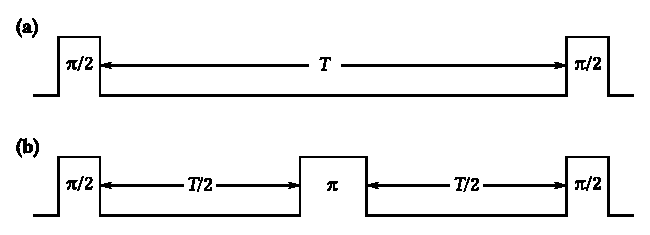
\includegraphics{figures_precreated/sequences.eps}}
    \caption[Timeline of Ramsey and spin echo experimental sequences]{
    Timeline of the experiment for \textbf{(a)} a regular Ramsey sequence, and \textbf{(b)} a Ramsey sequence with spin echo.}%endcaption
    \label{fig:bec-noise:visibility:sequences}
\end{figure}

The first protocol is a regular Ramsey sequence, depicted schematically in \figref{bec-noise:visibility:sequences},~(a): a $\pi/2$-pulse is applied by an electromagnetic coupler, creating a non-equilibrium superposition of components $\ket{1}$ and $\ket{2}$.
Mathematically, it means that coupling terms in~\eqnref{bec-noise:mean-field:cgpes-simplified} or in~\eqnref{bec-noise:wigner:single-particle-H} are enabled for a period of time equal to $t_{\mathrm{pulse}} = \theta / \Omega$, where $\theta = \pi/2$, with the Rabi frequency of the oscillator in this experiment being $\Omega = 2\pi \times 350\un{rad/s}$.
Since this pulse is short compared to the total evolution time, it was simulated via an application of the rotation matrix~\eqnref{bec-noise:mean-field:rotation-matrix}.

During the further evolution of the system the components experience complex dynamics, separating and merging periodically~\cite{Mertes2007}.
This, in turn, leads to periodic dephasing and self-rephasing of the \abbrev{bec} components.
After some period of the free evolution, a second $\pi/2$-pulse is applied, transforming the phase difference between the two components in the superposition into a population difference which can be measured through imaging of both \abbrev{bec} components.
Many such experiments are performed with different free evolution times, contributing one time-point each because the imaging effectively destroys the \abbrev{bec}.
A more detailed description of the experiment can be found in the paper by Egorov \textit{et~al}~\cite{Egorov2011}, and in his PhD thesis~\cite{Egorov2012}.
%acknowledgement
The experimental points used in this and the next section are also courtesy of M.~Egorov.

The simulations in this and the following sections used the plane wave basis (see \appref{bases} for details) and a $64\times8\times8$ spatial grid.
The integration was performed using a low-dissipation 4th-order Runge-Kutta algorithm (see \appref{numerical} for details).
This grid choice was made to ensure that mode populations were high, in view of the truncation approximation inherent in our method.

Coherence of the interference signal can be characterised by a common quantity~--- the fringe contrast, or visibility:
\begin{eqn}
\label{eqn:bec-noise:visibility:visibility}
    \mathcal{V}
    = \frac{2 \left| \int \langle \Psiop_1^\dagger \Psiop_2 \rangle \upd \xvec \right|}%
        {\int \langle \Psiop_1^\dagger \Psiop_1 + \Psiop_2^\dagger \Psiop_2 \rangle \upd \xvec},
\end{eqn}
where the denominator is just the total number of atoms in the system.
This quantity can be shown to be the envelope curve of the population fringes produced by the second $\pi/2$-pulse in the experiment.
In the mean-field model, the required correlations are calculated simply as
\begin{eqn}
    \tilde{n}
    & = \langle \Psiop_1^\dagger \Psiop_2 \rangle \approx \Psi_1^* \Psi_2, \\
    n_j
    & = \langle \Psiop_j^\dagger \Psiop_j \rangle \approx \Psi_j^* \Psi_j.
\end{eqn}
In the Wigner representation, we have to make the correlations symmetrically-ordered first, and then~\eqnref{wigner-bec:fpe-bec:moments} gives us
\begin{eqn}
    \tilde{n}
    & = \langle \Psiop_1^\dagger \Psiop_2 \rangle
    = \langle \symprod{ \Psiop_1^\dagger \Psiop_2 } \rangle
    \approx \Psi_1^* \Psi_2, \\
    n_j
    & = \langle \Psiop_j^\dagger \Psiop_j \rangle
    = \langle \symprod{ \Psiop_j^\dagger \Psiop_j }
        - \frac{\delta_{\restbasis_j}(\xvec, \xvec)}{2} \rangle
    \approx \pathavg{ \Psi_j^* \Psi_j } - \frac{M}{2V},
\end{eqn}
where we have used the fact that $\delta_{\restbasis_j}(\xvec, \xvec) \equiv M / V$ in the plane wave basis, where $M$ is the number of modes (for the grid we use $M = 64 \times 8 \times 8 = 4096$), and $V$ is the volume of the simulation area.

\begin{figure}
    \centerline{\includegraphics{figures_generated/bec_noise/ramsey_visibility_short.pdf}}

    \caption[Experimental and numerically simulated interferometric constrast in Ramsey sequence]{
    Comparison of experimental and numerically simulated interferometric contrast at the end of a regular Ramsey sequence with the evolution time $t$.
    Experimental results (black bars) are shown in comparison with the results given by the mean-field model (green dotted line), the truncated Wigner method (red dashed line), and the truncated Wigner with technical noises included (blue solid line).
    The mean-field results with losses turned off (yellow dash-dotted line) and the population-dependent visibility limit~\eqnref{bec-noise:visibility:limit} (grey dotted line) are included as a reference.}%endcaption

    \label{fig:bec-noise:visibility:ramsey-visibility}
\end{figure}

The visibility can serve as a good parameter of different effects (losses, quantum effects and technical noises) in the modelling of the experiment.
The inclusion of these factors in the simulation of the Ramsey sequence is demonstrated in~\figref{bec-noise:visibility:ramsey-visibility}.
The experimental results and their uncertainties are shown as the black bars in the figure.

The simplest model~--- the mean-field \abbrev{cgpe}s~\eqnref{bec-noise:mean-field:cgpes-simplified} with losses turned off~--- shows behavior that differs significantly from the experimental points: the visibility is completely restored during rephasings (yellow dash-dotted lines in the figure).
This is to be expected as the theoretical limit of visibility
\begin{eqn}
\label{eqn:bec-noise:visibility:limit}
    \mathcal{V}_{\mathrm{max}}
    = \frac{2 \sqrt{N_1 N_2}}{N_1 + N_2},
\end{eqn}
where $N_1$ and $N_2$ are populations before the second $\pi/2$-pulse, equals to $1$ in this case, and there are no other limiting factors.

\begin{figure}
    \centerline{%
    \includegraphics{figures_generated/bec_noise/ramsey_single_run_pop.pdf}%
    \includegraphics{figures_generated/bec_noise/echo_single_run_pop.pdf}}

    \caption[Component population in Ramsey and spin echo sequences]{
    Numerically simulated decay of the population of components $\ket{1}$ (blue solid lines) and $\ket{2}$ (red dashed lines) in \textbf{(a)} Ramsey and \textbf{(b)} spin echo sequences.}%endcaption

    \label{fig:bec-noise:visibility:population}
\end{figure}

However, in the experiment losses are present and are significantly asymmetrical as shown in~\figref{bec-noise:visibility:population},~(a).
With populations typical for the experiment (tens of thousands of atoms or less), the two-body loss process in $\ket{2}$ is significantly stronger than the three-body one in $\ket{1}$.
This makes the theoretical limit~\eqnref{bec-noise:visibility:limit} decrease with time, as the dotted grey line in~\figref{bec-noise:visibility:ramsey-visibility} illustrates.
The resulting mean-field prediction with the inclusion of nonlinear losses (green dotted lines) is much closer to the experimental data.

The application of the \abbrev{sde}s~\eqnref{bec-noise:wigner:sde} obtained with the Wigner method (red dashed lines) has little effect on the short-time visibility (although it becomes more important at longer times as we will see later in~\figref{bec-noise:visibility:visibility-long}).
The Wigner results can be further adjusted to account for the noise introduced by the final measurement and non-ideal coupling (blue solid lines), which will be explained in detail in the next section.

The final agreement with the experiment is still not ideal, and the explanation of this difference is an open question.
Potential unaccounted factors include finite temperature effects and interaction with the surrounding cloud of non-condensed atoms.

\begin{figure}
    \centerline{\includegraphics{figures_generated/bec_noise/echo_visibility_short.pdf}}

    \caption[Experimental and numerically simulated interferometric constrast in spin echo sequence]{
    Comparison of experimental and numerically simulated interferometric contrast at the end of a spin echo sequence with the evolution time $t$.
    Experimental results (black bars) show the final visibility value for a single spin echo sequence with the full evolution time $t$ as compared with the predictions from the mean-field model (green dotted line), the truncated Wigner method (red dashed line), and the truncated Wigner with technical noises included (blue solid line).}%endcaption

    \label{fig:bec-noise:visibility:echo-visibility}
\end{figure}

The asymmetricity introduced by the difference in loss rates can be compensated by periodically swapping the populations of the two components by a ``spin echo'' coupler pulse of the length $\pi$.
The simplest, yet already very effective, variant is to apply the $\pi$-pulse in the middle of the evolution as illustrated by~\figref{bec-noise:visibility:sequences},~(b).
With this additional pulse, by the end of a single experimental sequence the populations of two components become equal again as shown in~\figref{bec-noise:visibility:population},~(b), restoring the theoretical visibility limit~\eqnref{bec-noise:visibility:limit} back to $1$.

The mean-field model predicts the full recovery of the visibility even at long evolution times, which is inconsistent with the experiment as seen in~\figref{bec-noise:visibility:echo-visibility}.
On the other hand, the quasiprobability model qualitatively predicts the decay of visibility with time.
Just as in the case of the regular Ramsey sequence, the predictions of the simulation are improved by the inclusion of technical noise.

\begin{figure}
    \centerline{%
    \includegraphics{figures_generated/bec_noise/ramsey_visibility_long.pdf}%
    \includegraphics{figures_generated/bec_noise/echo_visibility_long.pdf}}

    \caption[Experimental and numerically simulated interferometric constrast in Ramsey and spin echo sequences for longer times]{
    Numerically simulated interferometric contrast for \textbf{(a)} a Ramsey sequence, and \textbf{(b)} a spin echo sequence at longer times.
    The results for the mean-field model (green dotted lines), the truncated Wigner method (red dashed lines) and the truncated Wigner with technical noises (blue solid lines) are plotted.}%endcaption

    \label{fig:bec-noise:visibility:visibility-long}
\end{figure}

The simulations can be performed for longer times as shown in~\figref{bec-noise:visibility:visibility-long}.
The difference between the mean-field and the truncated Wigner approach becomes clearer in~\figref{bec-noise:visibility:visibility-long},~(a), where the truncated Wigner predicts a significant decrease in the amplitude of the rephasing oscillations, caused by quantum noise.
One must remember though that at such times the simulated atom densities become too low due to losses and violate the truncation validity criterion~\eqnref{wigner-bec:truncation:delta-condition}, thus making the predictions less reliable.

% =============================================================================
\section{Phase noise}
% =============================================================================

Another important characteristic of a \abbrev{bec} interferometry experiment is the phase noise, which is connected with the visibility.
We will discuss it based on the same experiment~\cite{Egorov2011,Egorov2012} as in the previous section.

While in the simulation we can measure the visibility~\eqnref{bec-noise:visibility:visibility} simply by calculating a second-order moment, experimentalists do not have the luxury of knowing the wavefunctions of the components.
Instead, multiple runs of the Ramsey sequence with the same evolution time are performed, with the second $\pi/2$-pulse having a different phase lag $\phi$ each time.
The quantity that can be measured in the experiment is the normalized atom difference
\begin{eqn}
    P_z = \frac{N_2^\prime - N_1^\prime}{N_1^\prime + N_2^\prime},
\end{eqn}
where $N_1^\prime$ and $N_2^\prime$ are populations of the components obtained by imaging after the second $\pi/2$-pulse.
Using the rotation matrix~\eqnref{bec-noise:mean-field:rotation-matrix} it can be shown that $P_z$ can be expressed in terms of wave operators before the second $\pi/2$-pulse as
\begin{eqn}
    P_z(\phi)
    = - \frac{2}{N_1 + N_2} \Imag \left(
        e^{-i\phi} \int \langle \Psiop_1^\dagger \Psi_2 \rangle \upd\xvec
        \right).
\end{eqn}
One can notice that the integral of the second order moment in this expression is the same as in~\eqnref{bec-noise:visibility:visibility}, and is also normalized on the total population.
Therefore if we vary $\phi$ in the experiment, the resulting $P_z(\phi)$ can be fit with a sine function, and its maximum will give us the visibility $\mathcal{V}$.

\begin{figure}
    \centerline{%
    \includegraphics{figures_generated/bec_noise/illustration_noise_20ms.pdf}%
    \includegraphics{figures_generated/bec_noise/illustration_noise_450ms.pdf}}

    \caption{Phase noise in the experimental measurement of the visibility.
    Black dots illustrate }

    \label{fig:bec-noise:phase-noise:illustration}
\end{figure}

In practice, naturally, the measurement of $P_z$ is affected by various sources of technical noise.
As a result, the measured points are displaced in phase as compared to the ideal curve, and the width of this displacement $\omega$ is called the phase noise.
This is illustrated in~\figref{bec-noise:phase-noise:illustration} (the ``experimental'' points are taken from different simulation paths in the truncated Wigner simulation of the Ramsey sequence from the previous section).

In the experiment in question three such sources were identified.
First, the length of $\pi/2$-pulses varied throughout the exeprimental runs with an estimated standard deviation of $0.02\un{rad}$.
The phase lag $\phi$ also

\begin{figure}
    \centerline{\includegraphics{figures_generated/bec_noise/ramsey_noise.pdf}}

    \caption{Comparison of experimental and numerically simulated interferometric contrast in the Ramsey sequence.
    Plotted are the results obtained with the Wigner method (blue dashed line), Wigner method with the addition of the coupler noise (blue solid line), the noise introduced by the MW frequency instability (green dash-dotted line), the noise introduced by the imaging (red dotted line), and the combination of technical and quantum noises (black solid line), along with the experimental points (black bars).}

    \label{fig:bec-noise:phase-noise:ramsey-phnoise}
\end{figure}

\begin{figure}
    \centerline{\includegraphics{figures_generated/bec_noise/echo_noise.pdf}}

    \caption{Comparison of experimental and numerically simulated interferometric contrast in the spin echo sequence.
    Plotted are the results obtained with the Wigner method (blue dashed line), Wigner method with the addition of the coupler noise (blue solid line), the noise introduced by the MW frequency instability (green dash-dotted line), the noise introduced by the imaging (red dotted line), and the combination of technical and quantum noises (black solid line), along with the experimental points (black bars).}

    \label{fig:bec-noise:phase-noise:echo-phnoise}
\end{figure}

% =============================================================================
\section{Conclusion}
% =============================================================================

The examples in this chapter demonsrate that the truncated Wigner approach gives correct long-time predictions of quantum effects for the system comprised of large number of atoms.
Both of these features, large atom numbers and long time-scales, are essential to accurate interferometric measurements.
The predictions remains correct even despite multimode dynamical motion in three dimensions and substantial losses of most of the condensate atoms.
On longer time-scales, the experimental accuracy is limited by technical noises, and we have no data for comparisons.

